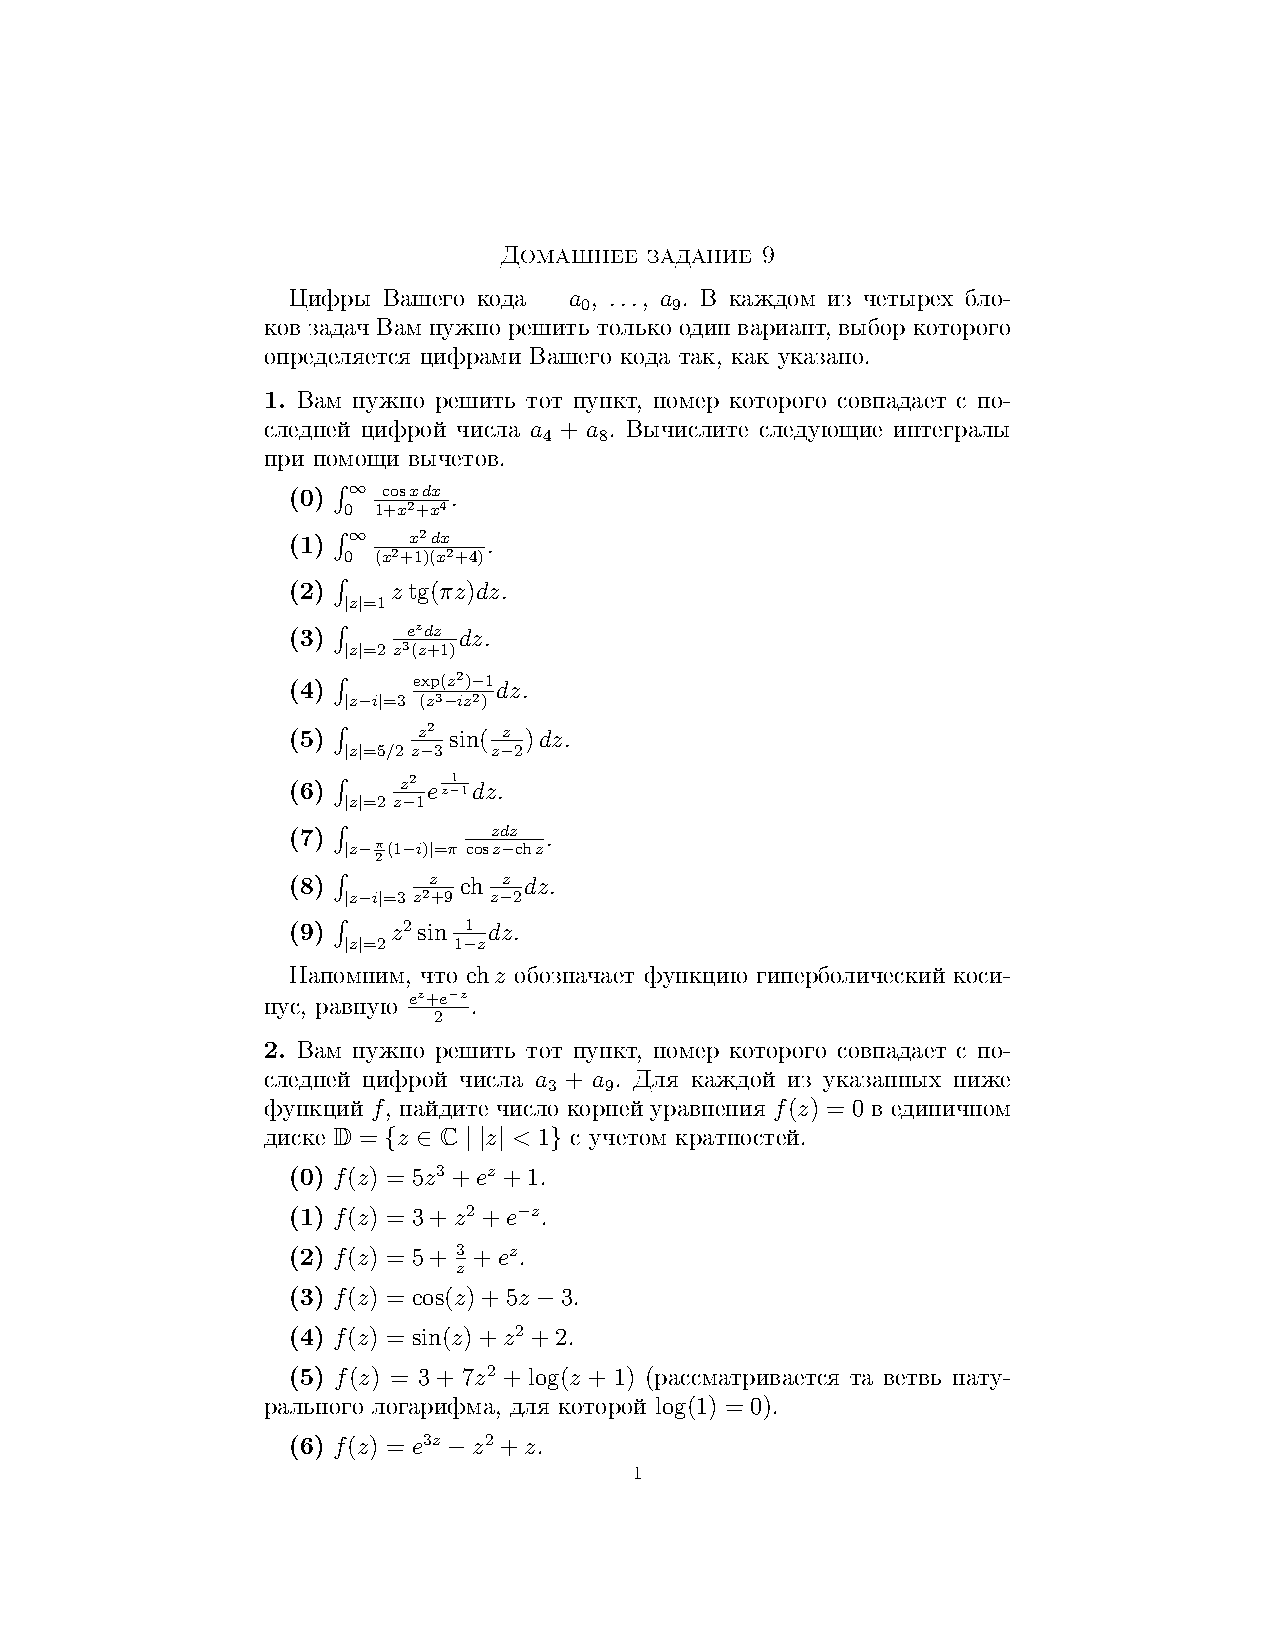
\includepdf[scale=1,pages=1-3]{Tasks/hw9}
\newpage
\section*{Решения}
\subsection*{Задача 1}
	Необходимо решить задачу $a_4 + a_8 = 7 + 8 = 5 \mod 10$
	\begin{gather*}
		\int_{|z| = \frac{5}{2}} \frac{z^2}{z-3} \sin\left(\frac{z}{z-2}\right) dz\\
		I = \int_{C} \frac{z^2}{z-3} \sin\left(\frac{z}{z-2}\right) dz,\ C: |z| = \frac{5}{2}\\
		I = 2 \pi i \sum \text{вычеты $f$ внутри контура}
	\end{gather*}
	Заметим, что особые точки это $z = 3$, но $|3| > \frac{5}{2}$. Следовательно $I = 2 \pi i * 0 = 0$, то есть интеграл равен $0$
\vskip 0.4in

\subsection*{Задача 2}
	Необходимо решить задачу $a_3 + a_9 = 9 + 6 = 5 \mod 10$
	\begin{gather*}
		f_1(z) = 3 +\log(z+1)\qquad f_2(z) = 7z^2\\
		|3+\log(z+1)|\leqslant 3 + |\log(z+1)|\\
		|\log(z+1)| = |\log|(z+1)| + i \arg(z+1)| \leqslant |\log|(z+1)||+ \pi \leqslant \log 2 + \pi < 4
	\end{gather*}
	Откуда $|3 + \log(z+1)| < 3 + 4 = 7$, при $|z| \to 1:\ |7z^2| \to 7$, откуда $|f_1(z)| < |f_2(z)|$ при $|z| = 1 - \epsilon$. Тогда по теореме Руше функции $f_2(z)$ и $f_1(z) + f_2(z)$ имеют равное количество нулей на $\mathbb{D}$, откуда у $f_1(z) + f_2(z)$ 2 нуля (так как у $f_2(z)$ 2 нуля).
\vskip 0.4in

\subsection*{Задача 3}
	Необходимо решить задачу $a_1 + a_9 = 7 + 6 = 3 \mod 10$
	$|f(e^{it})|>1$ для всех вещественных $t$, индекс $t \mapsto f(e^{it})$ относительно $0$ равен $1$, то $f(\mathbb{D}) \supset \mathbb{D}$
\vskip 0.4in

\subsection*{Задача 4}
	Необходимо решить задачу $a_4 + a_9 = 7 + 6 = 3 \mod 10$
	\begin{gather*}
		\text{V.p.}\int\limits_{-\infty}^{\infty} \frac{x^2 dx}{1 - x^4}
		= \lim_{R \to \infty} \int\limits_{-R}^{R} \frac{x^2}{1 - x^4}dx
		= \lim_{R \to \infty} \int\limits_{-R}^{R} -\frac{x^2}{(x-1)(x+1)(x^2+1)} dx\\
		= \lim_{R \to \infty}\left(
		\int\limits_{-R}^{-1} -\frac{x^2}{(x-1)(x+1)(x^2+1)} dx
		+ \int\limits_{-1}^{1} -\frac{x^2}{(x-1)(x+1)(x^2+1)} dx
		+ \int\limits_{1}^{R} -\frac{x^2}{(x-1)(x+1)(x^2+1)} dx \right)\\
		= \lim_{R \to \infty} (
		(-\frac{1}{4} \log(1+R) + \frac{1}{4}\log(-R+1) - \frac{1}{2} \tan^{-1}(R))
		- (-\frac{1}{4} \log(1+1) + \frac{1}{4}\log(-1+1) - \frac{1}{2} \tan^{-1}(-1))\\
		+ (-\frac{1}{4} \log(1+1) + \frac{1}{4}\log(-1+1) - \frac{1}{2} \tan^{-1}(-1))
		- (-\frac{1}{4} \log(1-1) + \frac{1}{4}\log(1+1) - \frac{1}{2} \tan^{-1}(1))\\
		+ (-\frac{1}{4} \log(1-1) + \frac{1}{4}\log(1+1) - \frac{1}{2} \tan^{-1}(1))
		- (-\frac{1}{4} \log(1-R) + \frac{1}{4}\log(R+1) - \frac{1}{2} \tan^{-1}(-R)))\\
		= \lim_{R \to \infty} (\tan^{-1}(-R) - \tan^{-1}(R))
		= -\pi 
	\end{gather*}

\begin{comment}
\subsection*{Задача 5}
	Необходимо решить задачу $a_0 + a_4 = 1 + 7 = 8 \mod 10$

\end{comment}